\documentclass[8pt,a4paper,compress]{beamer}

\usepackage{/home/siyer/lib/slides}

\title{Binary Search Trees}
\date{}

\begin{document}
\begin{frame}
\vfill
\titlepage
\end{frame}

\begin{frame}
\frametitle{Outline}
\tableofcontents
\end{frame}

\section{What is a Binary Search Tree (BST)?}
\begin{frame}[fragile]
\begin{itemize}
\item a binary tree is either empty or two disjoint binary trees (left and right)

\item a binary tree is in symmetric order if each node has a key and every node's key larger than all keys in its left subtree and smaller than all keys in its right subtree

\item a binary search tree (BST) is a binary tree in symmetric order

\begin{center}
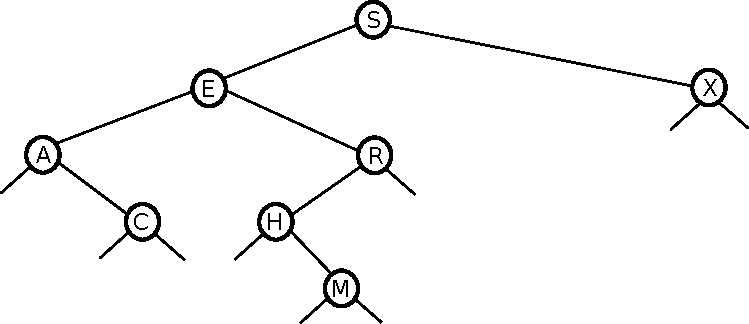
\includegraphics[scale=0.6]{{./figures/bst}.pdf}
\end{center}
\end{itemize}
\end{frame}

\begin{frame}[fragile]
\begin{itemize}
\item a BST representation in Java is a reference to a root node, which is composed of five fields: a key, a value, a reference to the left subtree, a reference to the right subtree, and the number of nodes in the subtree

\begin{lstlisting}[language=Java]
private class Node {
    private Key key; 
    private Value val; 
    private Node left, right; 
    private int N;

    public Node(Key key, Value val, int N) {
        this.key = key;
        this.val = val;
        this.N = N;
    }
}
\end{lstlisting}
\end{itemize}
\end{frame}

\section{Implementation of the Ordered Symbol Table API Using a BST}
\begin{frame}[fragile]
\begin{itemize}
\item basic operations
\begin{lstlisting}[language=Java]
public class BinarySearchTreeST<Key extends Comparable<Key>, Value> 
    implements OrderedST<Key, Value> {
    private Node root;

    private class Node { ... }
    
    public boolean isEmpty() { return size() == 0; }

    public int size() { return size(root); }

    private int size(Node x) {
        if (x == null) { return 0; }
        else return x.N;
    }

    public Value get(Key key) { return get(root, key); }

    private Value get(Node x, Key key) {
        if (x == null) { return null; }
        int cmp = key.compareTo(x.key);
        if      (cmp < 0) { return get(x.left, key); }
        else if (cmp > 0) { return get(x.right, key); }
        else              { return x.val; }
    }

    public boolean contains(Key key) { return get(key) != null; }
    ...
}
\end{lstlisting}
\end{itemize}
\end{frame}

\begin{frame}[fragile]
\begin{itemize}
\item basic operations (contd.)
\begin{lstlisting}[language=Java]
    ...
    public void put(Key key, Value val) {
        if (val == null) { delete(key); return; }
        root = put(root, key, val);
    }

    private Node put(Node x, Key key, Value val) {
        if (x == null) { return new Node(key, val, 1); }
        int cmp = key.compareTo(x.key);
        if      (cmp < 0) { x.left  = put(x.left,  key, val); }
        else if (cmp > 0) { x.right = put(x.right, key, val); }
        else              { x.val   = val; }
        x.N = 1 + size(x.left) + size(x.right);
        return x;
    }
    ...
\end{lstlisting}
\end{itemize}
\end{frame}

\begin{frame}[fragile]
\begin{itemize}
\item tree shape depends on order of insertion

\begin{minipage}{100pt}
\begin{center}
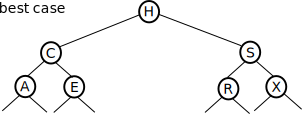
\includegraphics[scale=0.4]{{./figures/bst_possibility1}.pdf}
\end{center}
\end{minipage}%
\begin{minipage}{140pt}
\begin{center}
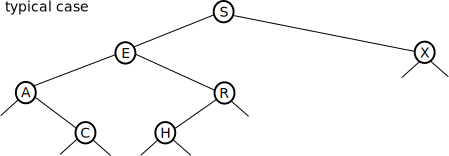
\includegraphics[scale=0.4]{{./figures/bst_possibility2}.pdf}
\end{center}
\end{minipage}%
\begin{minipage}{50pt}
\begin{center}
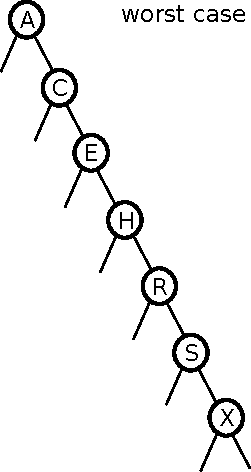
\includegraphics[scale=0.4]{{./figures/bst_possibility3}.pdf}
\end{center}
\end{minipage}

\item number of comparisons for search/insert is equal to 1 + depth of node

\item if $N$ distinct keys are inserted into a BST in random order,
the expected number of comparisons for a search/insert is $\sim 2\ln N$
\end{itemize}
\end{frame}

\begin{frame}[fragile]
\begin{itemize}
\item typical BST, built from 256 random keys

\begin{center}
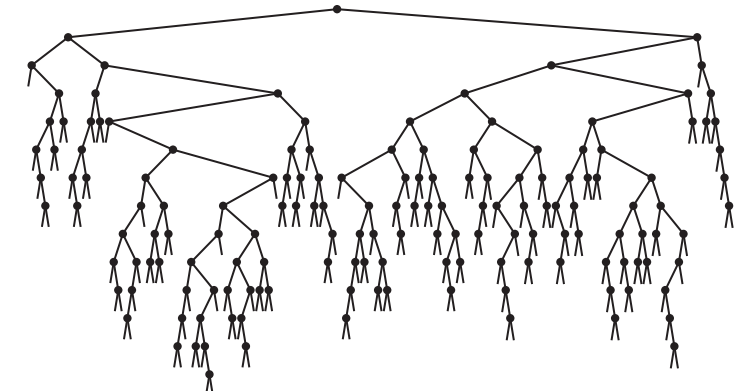
\includegraphics[scale=0.4]{{./figures/typical_bst}.png}
\end{center}
\end{itemize}
\end{frame}

\begin{frame}[fragile]
\begin{itemize}
\item minimum and maximum

\smallskip

\begin{center}
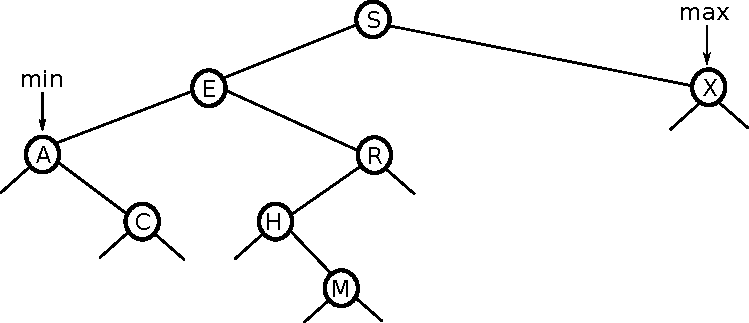
\includegraphics[scale=0.4]{{./figures/bst_min_max}.pdf}
\end{center}

\begin{lstlisting}[language=Java]
    ...
    public Key min() {
        if (isEmpty()) { return null; }
        return min(root).key;
    } 

    private Node min(Node x) { 
        if (x.left == null) { return x; }
        else                { return min(x.left); } 
    } 

    public Key max() {
        if (isEmpty()) { return null; }
        return max(root).key;
    } 

    private Node max(Node x) { 
        if (x.right == null) { return x; } 
        else                 { return max(x.right); } 
    } 
    ...
\end{lstlisting}
\end{itemize}
\end{frame}

\begin{frame}[fragile]
\begin{itemize}
\item floor and ceiling

\smallskip

\begin{center}
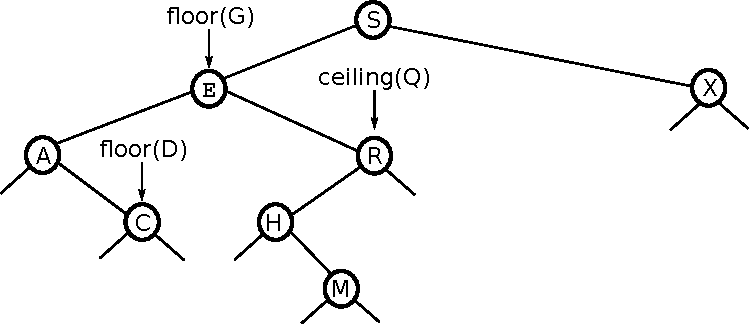
\includegraphics[scale=0.4]{{./figures/bst_floor_ceil}.pdf}
\end{center}

\smallskip

computing the floor of key $k$:
\begin{itemize}
\item case 1 ($k$ equals the key in the node): the floor of $k$ is $k$

\item case 2 ($k$ is less than the key in the node): the floor of $k$ is in the left subtree

\item case 3 ($k$ is greater than the key in the node): the floor of $k$ is in the right subtree if there is any key $\leq k$ in there; otherwise, it is the key in the node
\end{itemize}

\begin{lstlisting}[language=Java]
    ...
    public Key floor(Key key) {
        Node x = floor(root, key);
        if (x == null) { return null; }
        else           { return x.key; }
    } 

    private Node floor(Node x, Key key) {
        if (x == null) { return null; }
        int cmp = key.compareTo(x.key);
        if (cmp == 0) { return x; }
        if (cmp <  0) { return floor(x.left, key); }
        Node t = floor(x.right, key); 
        if (t != null) { return t; }
        else           { return x; } 
    } 
    ...
\end{lstlisting}
\end{itemize}
\end{frame}

\begin{frame}[fragile]
\begin{itemize}
\item floor and ceiling (contd.)

\smallskip

computing the ceiling of key $k$:
\begin{itemize}
\item case 1 ($k$ equals the key in the node): the ceiling of $k$ is $k$

\item case 2 ($k$ is greater than the key in the node): the ceiling of $k$ is in the right subtree

\item case 3 ($k$ is less than the key in the node): the ceiling of $k$ is in the left subtree if there is any key $\geq k$ in there; otherwise, it is the key in the node
\end{itemize}
\begin{lstlisting}[language=Java]
    ...
    public Key ceiling(Key key) {
        Node x = ceiling(root, key);
        if (x == null) { return null; }
        else           { return x.key; }
    }

    private Node ceiling(Node x, Key key) {
        if (x == null) { return null; }
        int cmp = key.compareTo(x.key);
        if (cmp == 0) { return x; }
        if (cmp > 0)  { return ceiling(x.right, key); }
        Node t = ceiling(x.left, key); 
        if (t != null) { return t; }
        else           { return x; }
    } 
    ...
\end{lstlisting}
\end{itemize}
\end{frame}

\begin{frame}[fragile]
\begin{itemize}
\item rank and selection

\begin{center}
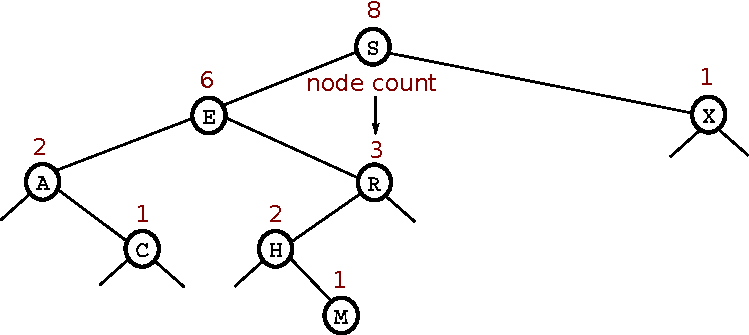
\includegraphics[scale=0.35]{{./figures/bst_rank_select}.pdf}
\end{center}

\begin{lstlisting}[language=Java]
    ...
    public int rank(Key key) { return rank(key, root); } 

    private int rank(Key key, Node x) {
        if (x == null) { return 0; }
        int cmp = key.compareTo(x.key); 
        if      (cmp < 0) { return rank(key, x.left); }
        else if (cmp > 0) { return 1 + size(x.left) + rank(key, x.right); }
        else              { return size(x.left); }
    } 

    public Key select(int k) {
        if (k < 0 || k >= size()) { return null; }
        Node x = select(root, k);
        return x.key;
    }

    private Node select(Node x, int k) {
        if (x == null) { return null; } 
        int t = size(x.left); 
        if      (t > k) { return select(x.left,  k); }
        else if (t < k) { return select(x.right, k - t - 1); } 
        else            { return x; }
    } 
    ...
\end{lstlisting}
\end{itemize}
\end{frame}

\begin{frame}[fragile]
\begin{itemize}
\item tree traversal
\begin{lstlisting}[language=Java]
public void preorder() { preorder(root); }

private void preorder(Node x) {
    if (x == null) { return; }
    process(x);
    preorder(x.left);
    preorder(x.right);
}
\end{lstlisting}

\begin{lstlisting}[language=Java]
public void inorder() { inorder(root); }

private void inorder(Node x) {
    if (x == null) { return; }
    inorder(x.left);
    process(x);
    inorder(x.right);
}
\end{lstlisting}

\begin{lstlisting}[language=Java]
public void postorder() { postorder(root); }

private void postorder(Node x) {
    if (x == null) { return; }
    postorder(x.left);
    postorder(x.right);
    process(x);
}
\end{lstlisting}

\item inorder traversal of a BST processes keys in ascending order
\end{itemize}
\end{frame}

\begin{frame}[fragile]
\begin{itemize}
\item range count and range search
\begin{lstlisting}[language=Java]
    ...
    public int size(Key lo, Key hi) {
        if (lo.compareTo(hi) > 0) { return 0; }
        if (contains(hi)) { return rank(hi) - rank(lo) + 1; }
        else              { return rank(hi) - rank(lo); }
    }

    public Iterable<Key> keys() {
        return keys(min(), max());
    }

    public Iterable<Key> keys(Key lo, Key hi) {
        LinkedQueue<Key> queue = new LinkedQueue<Key>();
        keys(root, queue, lo, hi);
        return queue;
    } 

    private void keys(Node x, LinkedQueue<Key> queue, Key lo, Key hi) { 
        if (x == null) { return; }
        int cmplo = lo.compareTo(x.key); 
        int cmphi = hi.compareTo(x.key); 
        if (cmplo < 0) { keys(x.left, queue, lo, hi); } 
        if (cmplo <= 0 && cmphi >= 0) { queue.enqueue(x.key); }
        if (cmphi > 0) { keys(x.right, queue, lo, hi); }
    } 
    ...
\end{lstlisting}
\end{itemize}
\end{frame}

\begin{frame}[fragile]
\begin{itemize}
\item deletion

\smallskip

to delete the minimum (maximum) key:
\begin{itemize}
\item go left (right) until you find a node with null left (right) link

\item replace that node by its right (left) link

\item update subtree counts

\end{itemize}
\begin{lstlisting}[language=Java]
    ...
    public void deleteMin() {
        if (isEmpty()) { throw new NoSuchElementException("ST underflow"); }
        root = deleteMin(root);
    }

    private Node deleteMin(Node x) {
        if (x.left == null) { return x.right; }
        x.left = deleteMin(x.left);
        x.N = size(x.left) + size(x.right) + 1; 
        return x;
    }

    public void deleteMax() {
        if (isEmpty()) { throw new NoSuchElementException("ST underflow"); }
        root = deleteMax(root);
    }

    private Node deleteMax(Node x) {
        if (x.right == null) { return x.left; }
        x.right = deleteMax(x.right);
        x.N = size(x.left) + size(x.right) + 1;
        return x;
    }   
    ...
\end{lstlisting}
\end{itemize}
\end{frame}

\begin{frame}[fragile]
\begin{itemize}
\item deletion (contd.)

\smallskip

to delete a node with key $k$ (Hibbard deletion), search for the node $t$ containing key $k$
\begin{itemize}
\item case 1 (0 children): delete $t$ by setting parent link to null

\item case 2 (1 child): delete $t$ by replacing parent link

\item case 3 (2 children): find successor $x$ of $t$ ($x$ has no left child); delete the minimum in $t$'s right subtree; and put $x$ in $t$'s spot
\end{itemize}
and update subtree counts

\begin{lstlisting}[language=Java]
    ...
    public void delete(Key key) {
        root = delete(root, key);
    }

    private Node delete(Node x, Key key) {
        if (x == null) { return null; }
        int cmp = key.compareTo(x.key);
        if      (cmp < 0) { x.left  = delete(x.left,  key); }
        else if (cmp > 0) { x.right = delete(x.right, key); }
        else { 
            if (x.right == null) { return x.left; }
            if (x.left  == null) { return x.right; }
            Node t = x;
            x = min(t.right);
            x.right = deleteMin(t.right);
            x.left = t.left;
        } 
        x.N = size(x.left) + size(x.right) + 1;
        return x;
    } 
    ...
\end{lstlisting}
\end{itemize}
\end{frame}

\section{Performance Characteristics}
\begin{frame}[fragile]
\begin{itemize}
\item symbol table operations summary
\begin{center}
\begin{tabular}{cccc}
\textbf{operation} & \textbf{unordered linked list} & \textbf{ordered array} & \textbf{BST} \\ \hline \\
search & $N$ & $\lg N$ & $h^\dagger$ \\
insert & $N$ & $N$ & $h$ \\
delete & $N$ & $N$ & $N^{\dagger\dagger}$ \\
min/max & - & 1 & $h$ \\
floor/ceiling & - & $\lg N$ & $h$\\
rank & - & $\lg N$ & $h$ \\
select & - & 1 & $h$ \\
ordered iteration & - & $N$ & $N$ 
\end{tabular} 

\bigskip

\tiny $\dagger$ $h$ is the height of BST, proportional to $\log N$ if keys inserted in random order

$\dagger\dagger$ $\sqrt{N}$ in the average case; other operations also become $\sqrt{N}$ if deletions are allowed
\end{center}
\end{itemize}
\end{frame}
\end{document}
